\documentclass[a4paper,12pt]{article}
\usepackage{graphicx}
\usepackage{amsmath,amssymb}
\usepackage{listings}
\usepackage{xcolor}
\usepackage{tikz}
\usepackage{caption}
\usepackage{hyperref}
\usepackage{tocloft}

\title{Arduino-Based Digital Clock with Timer Mode}
\author{Dwarak A - EE24BTECH11019}
\date{\today}

\begin{document}

\maketitle

\begin{abstract}
This report describes the design and implementation of an Arduino-based digital clock with an integrated timer mode. The system utilizes a 7447 BCD to 7-segment decoder with common anode (active low) 7-segment displays and button-based controls for time adjustments. Timekeeping is managed via a timer interrupt, while the display is driven using multiplexing to handle six digits representing hours, minutes, and seconds.
\end{abstract}

\section{Introduction}
Digital clocks play a crucial role in embedded systems. This project implements an Arduino-based clock that displays time in hours, minutes, and seconds while providing a countdown timer mode. Key features include the use of a 7447 BCD to 7-segment decoder (designed for common anode displays, meaning the segment outputs are active low), multiplexed display control, and several pushbuttons for user interaction.

\section{Hardware Setup}
\subsection{Components Required}
 \begin{table}[h!]
    \centering
    \begin{tabular}{|c|c|}
        \hline
        \textbf{One end of Jumper Wire}  & \textbf{Another end of Jumper Wire} \\
        \hline
          Digital pin 0 & Push button 16 \\
          Digital pin 1 & Push button 17 \\
          Digital pin 2 & LCD pin 4 \\
          Digital pin 3 & LCD pin 6 \\
          Digital pin 4 & LCD pin 11 \\
          Digital pin 5 & LCD pin 12 \\
          Digital pin 6 & LCD pin 13 \\
          Digital pin 7 & LCD pin 14 \\
          Digital pin 8 & Push button 18 \\
          Digital pin 9 & Push button 19 \\
          Digital pin 10 & Push button 20 \\
          Digital pin 11 & Push button 21 \\
          Digital pin 12 & Push button 22 \\
          Digital pin 13 & Push button 23 \\
          Analog pin A1 & Push button 15 \\
          Analog pin A2 & Push button 14 \\
          Analog pin A3 & Push button 13 \\
          Analog pin A4 & Push button 12 \\
          Analog pin A5 & Push button 11 \\
          Analog pin A0 & Push buttons 1-10 (digit buttons)\\
          LCD pin 1 & Ground \\
          LCD pin 2 & 5V \\
          LCD pin 15 & 5V via 1k $\Omega$ resistor \\
          LCD pin 16 & Ground \\
          LCD pin 3 & Ground via 1.5 k $\Omega$ resistor \\
          LCD pin 5 & Ground \\
          LCD pin 5 & All push buttons \\
          
        \hline
    \end{tabular}
\end{table}
\newpage

\subsection{Basic Connections}

\subsubsection{BCD Outputs to 7447 Decoder}
The Arduino outputs BCD values on digital pins PD2--PD5, which are fed into the 7447 decoder. Since the displays are common anode, the decoder outputs are active low. The connections are shown in Table~\ref{tab:7447}.
 \begin{table}[h!]
    \centering
    \begin{tabular}{|c|c|}
        \hline
        \textbf{Button number}  & \textbf{Function} \\
        \hline
           1 - 10 & Digits 0 - 9 \\
           11 & Clear \\
           12 & $\ln{(x)}$ and $\log{(x)}$ \\
           13 & Right Parenthesis \\
           14 & $\sin{(x)}$, $\cos{(x)}$, and $\tan{(x)}$ \\
           15 & $e$ and $\pi$ \\
           16 & Backspace \\
           17 & Decimal Point \\
           18 & Equal To \\
           19 & Left Parenthesis \\
           20 & Division (/)\\
           21 & Multiplications (*)\\
           22 & Subtraction(-) \\
           23 & Addition (+) \\
        \hline
    \end{tabular}
\end{table}


\subsubsection{Multiplexed 7-Segment Displays}
To display six digits using limited Arduino pins, multiplexing is employed. The Arduino sequentially activates each digit by driving its enable pin. The digit connections are listed in Table~\ref{tab:multiplex}.
\begin{table}[h]
    \centering
    \begin{tabular}{|c|c|c|c|}
        \hline
        \textbf{Display} & \textbf{Arduino Pin} & \textbf{ATmega328P Pin} & \textbf{Function} \\
        \hline
        DISP1 & PD6 & 10 & Selects Hour Tens display \\
        DISP2 & PD7 & 11 & Selects Hour Units display \\
        DISP3 & PB0 & 8  & Selects Minute Tens display \\
        DISP4 & PB1 & 9  & Selects Minute Units display \\
        DISP5 & PB2 & 10 & Selects Second Tens display \\
        DISP6 & PB3 & 11 & Selects Second Units display \\
        \hline
    \end{tabular}
    \caption{7-Segment Display Selection}
    \label{tab:display_selection}
\end{table}


\subsubsection{Pushbutton Connections}
The pushbuttons, connected using the Arduino's internal pull-up resistors, pull the corresponding input LOW when pressed. Their connections are given in Table~\ref{tab:buttons}.
\begin{table}[h]
    \centering
    \begin{tabular}{|c|c|c|c|}
        \hline
        \textbf{Button} & \textbf{Arduino Pin} & \textbf{ATmega328P Pin} & \textbf{Function} \\
        \hline
        HOUR\_BUTTON   & PB4 & 12 & Increments the hour \\
        MIN\_BUTTON    & PC0 & A0 & Increments the minute \\
        SEC\_BUTTON    & PC1 & A1 & Increments the second \\
        \hline
    \end{tabular}
    \caption{Push Button Connections}
    \label{tab:push_buttons}
\end{table}


\section{Arduino to AVR Pin Mapping}
The following table shows how the Arduino board’s pin labels correspond to the AVR microcontroller’s port names as referenced in AVR GCC. This mapping is essental for low-level programming and direct port manipulation.
\begin{table}[h]
    \centering
    \begin{tabular}{|c|c|}
        \hline
        \textbf{Arduino Pin} & \textbf{AVR Pin/Port} \\
        \hline
        D2  & PD2 \\
        D3  & PD3 \\
        D4  & PD4 \\
        D5  & PD5 \\
        D6  & PD6 \\
        D7  & PD7 \\
        D8  & PB0 \\
        D9  & PB1 \\
        D10 & PB2 \\
        D11 & PB3 \\
        A0  & PC0 \\
        A1  & PC1 \\
        A2  & PC2 \\
        A3  & PC3 \\
        A5  & PC5 \\
        \hline
    \end{tabular}
    \caption{Mapping of Arduino Pins to AVR GCC Pin Terms}
    \label{tab:avr_mapping}
\end{table}



\section{IC and Display Pinouts}
\subsection{7-Segment Display Pinout}
\begin{center}
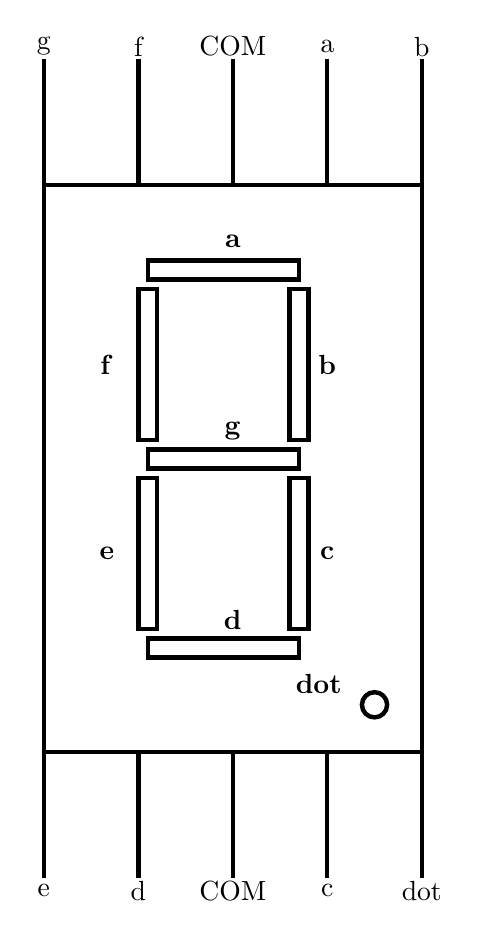
\begin{tikzpicture}
  [
    scale=0.8,
    >=stealth,
    point/.style = {draw, circle,  fill = black, inner sep = 0.5pt},
    dot/.style   = {draw, circle,  fill = black, inner sep = .2pt},
  ]

%Vertices of the main display rectangle
\def \xmin{0}
\def \xmax{6}
\def \ymin{0}
\def \ymax{-9}

%Number of pins on a side
\def \n{5}
\def \k{1.6}

%Draw the display rectangle
\draw[ultra thick] (\xmin,\ymin)rectangle (\xmax,\ymax);

%Define height of pins and their separation
\def \height{2}
\pgfmathsetmacro{\wid}{(\xmax-\xmin)/(\n-1)}

%Defining y axis divisions
\pgfmathsetmacro{\ywid}{(\ymin-\ymax)/(\n-2)}

\foreach \i in {0,...,4}
{
\draw[ultra thick] (\xmin + \i*\wid, \ymin) -- (\xmin + \i*\wid, \ymin + \height); 
\draw[ultra thick] (\xmin + \i*\wid, \ymax) -- (\xmin + \i*\wid, \ymax -\height); 
}
%%
%%%
\foreach [count=\i] \j in {g,f,COM,a,b}{
            \node (\i) at ( -1.5 + \i*\wid,\height+0.2) {\j} ;
            }
\foreach [count=\i] \j in {e,d,COM,c,dot}{
            \node (\i) at ( -1.5 + \i*\wid,\ymax -\height-0.2) {\j} ;
            }

\foreach [count=\i] \j in {\textbf{a},\textbf{g},\textbf{d}}
{            
\draw[ultra thick] (\xmin+1.1*\wid,{\ymin-(\i-0.5)*\ywid} ) rectangle +(\k*\wid,0.3 );
\node (\i) at ( \xmin + 2*\wid,{\ymin-(\i-0.7)*\ywid}) {\j} ;
}
\foreach [count=\i] \j in {\textbf{f},\textbf{e}}
{            
\draw[ultra thick] (\xmin+\wid,{\ymin-(\i+0.35)*\ywid} ) rectangle +(0.3,\k*\wid );
\node (\i) at ( \xmin + \wid-0.5,{\ymin-(\i-0.05)*\ywid}) {\j} ;
}
\foreach [count=\i] \j in {\textbf{b},\textbf{c}}
{            
\draw[ultra thick] (\xmin+2.6*\wid,{\ymin-(\i+0.35)*\ywid } ) rectangle +(0.3,\k*\wid );
\node (\i) at ( \xmin + 3*\wid,{\ymin-(\i-0.05)*\ywid}) {\j} ;
}


%
\draw[ultra thick] (\xmax - 0.5*\wid,{\ymax+0.25*\ywid}) circle [radius=0.2];
\draw[ultra thick](\xmax - 0.5*\wid,{\ymax+0.25*\ywid}) node[sloped, anchor=center, above, text width=2.0cm]{\textbf{dot}};    
\end{tikzpicture}


\captionof{figure}{7-Segment Display Pinout (Common Anode, Active Low)}
\label{fig:7seg}
\end{center}

\subsection{7447 Decoder Pinout}
Below is the placeholder for your TikZ picture for the 7447 decoder pinout. Insert your TikZ code here.

\begin{figure}[h]
    \centering
    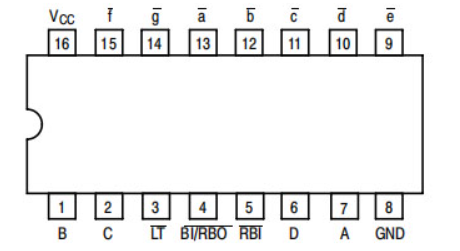
\includegraphics[width=0.8\textwidth]{figs/7447_pinout.png}
    \caption{7447 IC Pinout Diagram}
    \label{fig:7447_pinout}
\end{figure}

\section{Multiplexing Explanation}
Multiplexing is employed to drive multiple 7-segment displays using a limited number of Arduino pins. The process is as follows:
\begin{enumerate}
    \item The Arduino sets the BCD outputs (PD2--PD5) to the binary value corresponding to the digit to be displayed.
    \item It then activates the corresponding digit enable pin (one of pins 6--11) for a brief period (of the order $10^{-3}$ s).
    \item The digit is then deactivated, and the Arduino moves to the next digit.
\end{enumerate}
This rapid cycling (typically at least 50 Hz per digit) creates the illusion of all digits being lit simultaneously, due to persistence of vision.

\section{Timekeeping with Timer Interrupt}
The Arduino utilizes Timer0 to generate an interrupt every 1 ms. This interrupt increments a global millisecond counter. When the counter reaches 1000, indicating one second has elapsed, the following steps occur:
\begin{itemize}
    \item The seconds value is incremented.
    \item When seconds reach 60, they reset to 0 and the minutes counter is incremented.
    \item Similarly, when minutes reach 60, the hours counter is incremented.
    \item When hours reach 24, the clock resets to 00:00:00.
\end{itemize}

\section{Button Functions}
\subsection{Increment Buttons (A0--A2)}
\begin{itemize}
    \item \textbf{Short press}: Increments the corresponding time unit (hour, minute, or second).
    \item \textbf{Long press (after 2 seconds)}: Initiates continuous incrementing at a rate of one increment every 200 ms.
\end{itemize}

\subsection{Pause/Play Button (A3)}
\begin{itemize}
    \item \textbf{Short press}: Toggles between pause and play states.
    \item \textbf{Long press (after 5 seconds)}: Resets the active mode's time to 00:00:00 and pauses the clock.
\end{itemize}

\subsection{Clock/Timer Mode Toggle (A5)}
Pressing the mode toggle button switches between clock mode (count-up) and timer mode (count-down) without losing the stored time for either mode.

\section{Source Code}
For easy access to the complete source code of this project, visit the following repository:
\begin{center}
    \url{https://github.com/Dwarak-A/EE1003/blob/main/hardware/clock}
\end{center}

\section{Conclusion}
This project demonstrates the implementation of an Arduino-based digital clock featuring a timer mode. By utilizing a 7447 BCD to 7-segment decoder with common anode displays (active low) and employing multiplexing, the design efficiently drives a six-digit display. The use of timer interrupts ensures accurate timekeeping, and the system allows user interaction through multiple pushbuttons.

\end{document}
